%%%%%%%%%%%%%%%%%%%%%%%%%%%%%%% beamer %%%%%%%%%%%%%%%%%%%%%%%%%%%%%%%%%%%%%%%%%%%%%%%%%
% To run - pdflatex filename.tex
%      acroread filename.pdf
%%%%%%%%%%%%%%%%%%%%%%%%%%%%%%%%%%%%%%%%%%%%%%%%%%%%%%%%%%%%%%%%%%%%%%%%%%%%%%%%%%%%%%%%

\documentclass[compress,oilve]{beamer}
\mode<presentation>

\usetheme[]{CambridgeUS}
% other themes: AnnArbor, Antibes, Bergen, Berkeley, Berlin, Boadilla, boxes, CambridgeUS, Copenhagen, Darmstadt, default, Dresden, Frankfurt, Goettingen,
% Hannover, Ilmenau, JuanLesPins, Luebeck, Madrid, Maloe, Marburg, Montpellier, PaloAlto, Pittsburg, Rochester, Singapore, Szeged, classic

\usecolortheme{beaver}
% color themes: albatross, beaver, beetle, crane, default, dolphin,  fly, lily, orchid, rose, seagull, seahorse, sidebartab, whale, wolverine

\usefonttheme{professionalfonts}
% font themes: default, professionalfonts, serif, structurebold, structureitalicserif, structuresmallcapsserif


\hypersetup{pdfpagemode=FullScreen} % makes your presentation go automatically to full screen

% define your own colors:
\definecolor{Red}{rgb}{1,0,0}
\definecolor{Blue}{rgb}{0,0,1}
\definecolor{Green}{rgb}{0,1,0}
\definecolor{magenta}{rgb}{1,0,.6}
\definecolor{lightblue}{rgb}{0,.5,1}
\definecolor{lightpurple}{rgb}{0.8, 0.6, 0.9}
\definecolor{gold}{rgb}{.6,.5,0}
\definecolor{orange}{rgb}{1,0.4,0}
\definecolor{hotpink}{rgb}{1,0,0.5}
\definecolor{newcolor2}{rgb}{.5,.3,.5}
\definecolor{newcolor}{rgb}{0,.3,1}
\definecolor{newcolor3}{rgb}{1,0,.35}
\definecolor{darkgreen1}{rgb}{0, .35, 0}
\definecolor{darkgreen}{rgb}{0, .6, 0}
\definecolor{darkred}{rgb}{.75,0,0}
\definecolor{skyblue}{HTML}{75bbfd}

\definecolor{olive}{cmyk}{0.64,0,0.95,0.4}
\definecolor{purpleish}{cmyk}{0.75,0.75,0,0}

% can also choose different themes for the "inside" and "outside"

% \usepackage{beamerinnertheme_______}
% inner themes include circles, default, inmargin, rectangles, rounded

% \usepackage{beamerouterthemesmoothbars}
% outer themes include default, infolines, miniframes, shadow, sidebar, smoothbars, smoothtree, split, tree


\useoutertheme[subsection=true, height=40pt]{smoothbars}

% to have the same footer on all slides
%\setbeamertemplate{footline}[text line]{STUFF HERE!}
\setbeamertemplate{footline}[text line]{} % makes the footer EMPTY
% include packages
%

%show the page numbers in footnote
%\addtobeamertemplate{navigation symbols}{}{%
%	\usebeamerfont{footline}%
%	\usebeamercolor[fg]{footline}%
%	\hspace{1em}%
%	\insertframenumber/\inserttotalframenumber
%}

\setbeamercolor{footline}{fg=purpleish}
\setbeamerfont{footline}{series=\bfseries}

%add color to curent subsection
\setbeamertemplate{section in head/foot}{\hfill\tikz\node[rectangle, fill=darkred, rounded corners=1pt,inner sep=1pt,] {\textcolor{white}{\insertsectionhead}};}
\setbeamertemplate{section in head/foot shaded}{\textcolor{darkred}{\hfill\insertsectionhead}}

% Remove bullet of subsections
\setbeamertemplate{headline}
{%
	\begin{beamercolorbox}{section in head/foot}
		\insertsectionnavigationhorizontal{\textwidth}{}{}
	\end{beamercolorbox}%
}


% modify headlline, specially headline size
\setbeamertemplate{headline}{%
	\leavevmode%
	\hbox{%
		\begin{beamercolorbox}[wd=\paperwidth,ht=3.5ex,dp=1.125ex]{palette quaternary}%
			\insertsectionnavigationhorizontal{\paperwidth}{}{\hskip0pt plus1filll}
		\end{beamercolorbox}%
	}
}

\setbeamertemplate{footline}{%
	\leavevmode%
	\hbox{\begin{beamercolorbox}[wd=.5\paperwidth,ht=2.5ex,dp=1.125ex,leftskip=.3cm plus1fill,rightskip=.3cm]{author in head/foot}%
			\usebeamerfont{author in head/foot}\insertshortauthor ~ \insertshortinstitute
		\end{beamercolorbox}%
		\begin{beamercolorbox}[wd=.5\paperwidth,ht=2.5ex,dp=1.125ex,leftskip=.3cm,rightskip=.3cm plus1fil]{title in head/foot}%
			\usebeamerfont{title in head/foot}\insertshorttitle\hfill\insertframenumber\,/\,\inserttotalframenumber
	\end{beamercolorbox}}%
	\vskip0pt%
}

\usepackage{xcolor}
\definecolor{keywords}{rgb}{.224,.451,.686}

\newcommand{\tc}[2]{
	\textcolor{#1}{\textbf{#2}}
}

%\setbeamertemplate{navigation symbols}{}

\title{Support Vector Machines}
\author{ML Instruction Team, Fall 2022}
\institute[]{CE Department \newline  Sharif University of Technology \newline \newline \newline
	Ali Sharifi-Zarchi \newline
	Behrooz Azarkhalili \newline
	Alireza Gargoori Motlagh}
\date[\today]{}
%\titlegraphic{\includegraphics[scale=.35]{example-image}}



%Write \usepackage{etex} just after the \documentclass line (it should be the first loaded package).
\usepackage{etex}
\usepackage{subcaption}
\usepackage{caption}
\usepackage{multicol}
\usepackage{amsmath}
\usepackage{epsfig}
\usepackage{graphicx}
\usepackage{amsmath}
\usepackage[all,knot]{xy}
\xyoption{arc}
\usepackage{url}
\usepackage{multimedia}
\usepackage{hyperref}
\hypersetup{colorlinks,linkcolor=blue,citecolor=redorange,urlcolor=darkred}
\usepackage{multirow}
\usepackage[font={scriptsize}]{caption}
\usepackage{pgf}
\usepackage{fontspec}
%\setsansfont[Scale=MatchLowercase, BoldFont = * Bold, ItalicFont = * Italic]{Caladea}

%\usepackage{enumitem,xcolor}
%\newcommand{\labelitemi}{$\blacksquare$}
%\newcommand{\labelitemii}{$\diamond$}
%\newcommand{\labelitemiii}{$\square$}
%\newcommand{\labelitemiv}{$\ast$}
%\setbeamercolor*{item}{fg=red}


\usefonttheme{professionalfonts} 
\setbeamertemplate{itemize item}{\color{skyblue}$\blacksquare$}
\setbeamertemplate{itemize subitem}{\color{hotpink}$\blacktriangleright$}
\setbeamertemplate{itemize subsubitem}{\color{orange}$\bullet$}


\usepackage{anyfontsize}
\usepackage{t1enc}
\usepackage{tikz}
\usetikzlibrary{calc,trees,positioning,arrows,chains,shapes.geometric,decorations.pathreplacing,decorations.pathmorphing,shapes,matrix,shapes.symbols}



\newtheorem{proposition}[theorem]{Proposition}
\newtheorem{remark}[theorem]{Remark}
\newtheorem{assumption}[theorem]{Assumption}

\usepackage{fontspec,unicode-math}
\setmainfont[Scale=0.9]{Consolas}
%\setmonofont[Scale=0.9]{Monaco}
\setsansfont[Scale=1]{Times New Roman}


%\usepackage{smartdiagram}
%\usesmartdiagramlibrary{additions}
%%%%%%%%%%%%%%%%%%%%%%%%%%%%%%%%%%%%%%%%%%%%%%%%%%%%%%%%%%%%%%%%%%%%%%%%%%%%%%%%%%%%%%%%%%%%
%%%%%%%%%%%%%%%%%%%%%%%%%%%%%% Title Page Info %%%%%%%%%%%%%%%%%%%%%%%%%%%%%%%%%%%%%%%%%%%
%%%%%%%%%%%%%%%%%%%%%%%%%%%%%%%%%%%%%%%%%%%%%%%%%%%%%%%%%%%%%%%%%%%%%%%%%%%%%%%%%%%%%%%%%%


%%%%%%%%%%%%%%%%%%%%%%%%%%%%%%%%%%%%%%%%%%%%%%%%%%%%%%%%%%%%%%%%%%%%%%%%%%%%%%%%%%%%%%%%%%
%%%%%%%%%%%%%%%%%%%%%%%%%%%%%% Begin Your Document %%%%%%%%%%%%%%%%%%%%%%%%%%%%%%%%%%%%%%%
%%%%%%%%%%%%%%%%%%%%%%%%%%%%%%%%%%%%%%%%%%%%%%%%%%%%%%%%%%%%%%%%%%%%%%%%%%%%%%%%%%%%%%%%%%
\begin{document}
	
	%%%%%%%%%%%%%%%%%%%%%%%%%%%%%%%%%%%%%%%%%%%%%%%%%%%%%%%%%%%%%%%%%%%%%%%%%%%%%%%%%%%%%%%%%%
	\fontsize{9}{9}
	\begin{frame}[noframenumbering, plain]
		\titlepage
	\end{frame}
	
	%%%%%%%%%%%%%%%%%%%%%%%%%%%%%%%%%%%%%%%%%%%%%%%%%%%%%%%%%%%%%%%%%%%%%%%%%%%%%%%%%%%%%%%%%%
	\section{Introduction}
	%%%%%%%%%%%%%%%%%%%%%%%%%%%%%%%%%%%%%%%%%%%%%%%%%%%%%%%%%%%%%%%%%%%%%%%%
	%%%%%%%%%%%%%%%%%%%%%%%%%%%%%%%%%%%%%%%%%%%%%%%%%%%%%%%%%%%%%%%%%%%%%%%%%%%%%%%%%%%%%%%%%%%%
	\frame{\frametitle{Hyperplane}
		
		
		\begin{itemize}
			\item \tc{keywords}{Hyperplane}: A hyperplane in \textit p dimensions is an affine subspace of dimension \textit {p-1}:
			
			$$\beta_0 + \beta_1 X_1 + \beta_2 X_2 + ... + \beta_p X_p = 0$$ 
			\begin{figure}
				\centering
				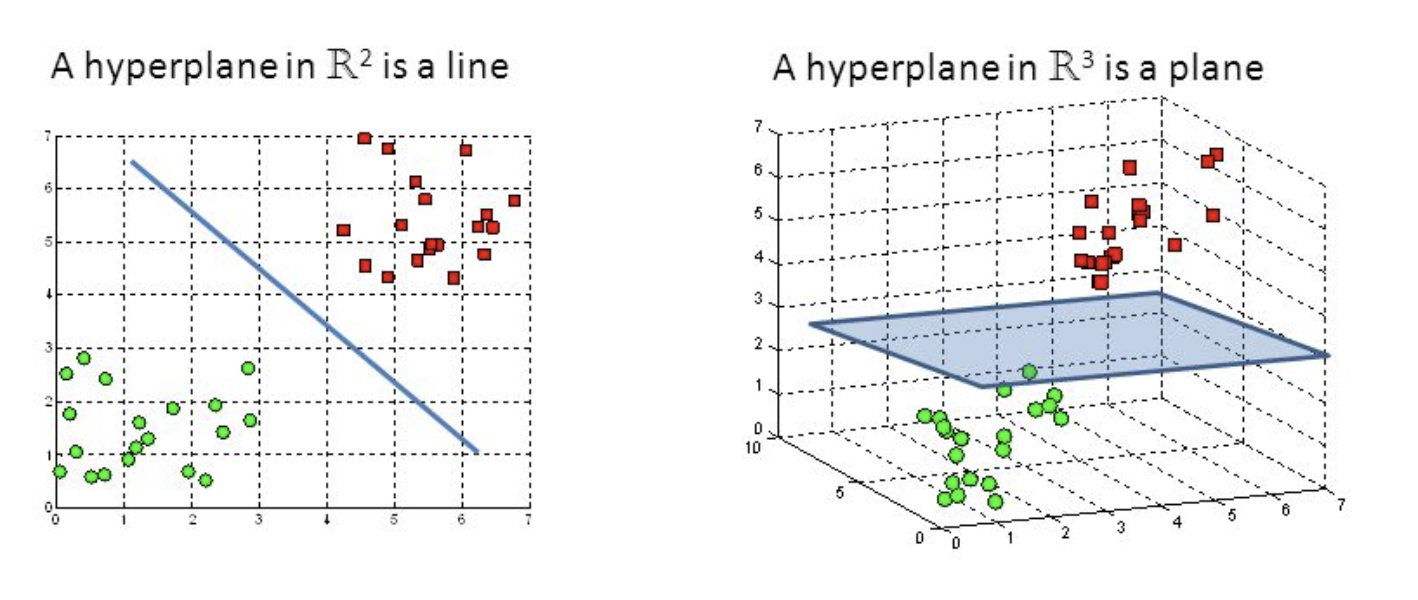
\includegraphics[scale=0.15]{Figs/hyperplane.png}
				\caption{Hyperplanes, \href{https://www.ai-summary.com/summary-hyperplane/}{Source}}
			\end{figure}
			
			\item The vector $\beta = (\beta_1, \beta_2, ..., \beta_p)$ is called the \tc{keywords}{normal vector} -- it points in a direction orthogonal to the surface of the defined hyperplane. \newline 
			
			\item If $f(X) = \beta_0 + \beta_1 X_1 + \beta_2 X_2 + ... + \beta_p X_p = \beta^T X + \beta_0$, then $f(X)$ divides the \textit p-dimensional feature space into two half-spaces. %($f(X) > 0$ for one side and $f(X) < 0$ for the other side). %\newline \newline
			
			\item So if we code $Y^{(i)} \in \{\pm 1\}$, then $\forall i: \quad Y^{(i)}f(X^{(i)}) > 0$
		\end{itemize}	
		
	}


	\frame{\frametitle{Intuition: Margins}
		
		\begin{itemize}
			\item Separating Hyperplane
			\begin{figure}
				\centering
				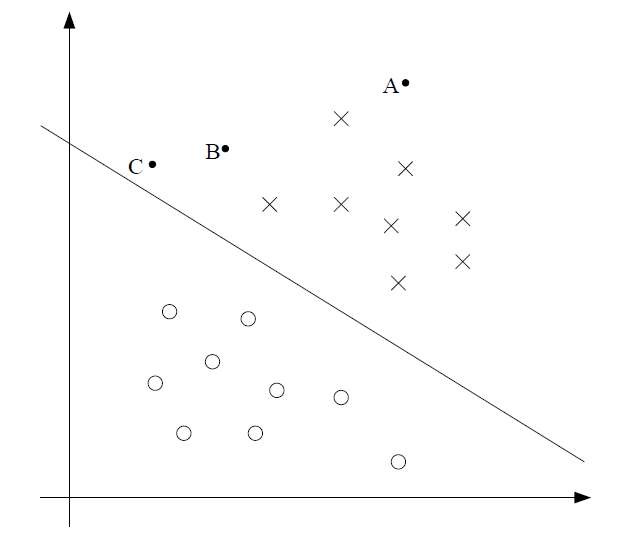
\includegraphics[scale=0.4]{Figs/separating_hyperplane.png}
				\caption{Separating Hyperplane, \href{http://cs229.stanford.edu/lectures-spring2022/main_notes.pdf}{Source}}
			\end{figure}
			
			\item 
			Our confidence about the prediction of classes of A, B and C relies on their \tc{keywords}{distance from decision boundary}. \newline
			
			\item 
			We try to find the optimal hyperplane that separates the classes in the feature space.
		\end{itemize}	
		
	}
	
	
	%%%%%%%%%%%%%%%%%%%%%%%%%%%%%%%%%%%%%%%%%%%%%%%%%%%%%%%%%%%%%%%%%%%
	\section{Maximal Margin Classifier}
	%%%%%%%%%%%%%%%%%%%%%%%%%%%%%%%%%%%%%%%%%%%%%%%%%%%%%%%%%%%%%%%%%%%
	\frame{\frametitle{Maximal Margin Classifier}
		
		\begin{itemize}
	
			\begin{figure}
				\centering
				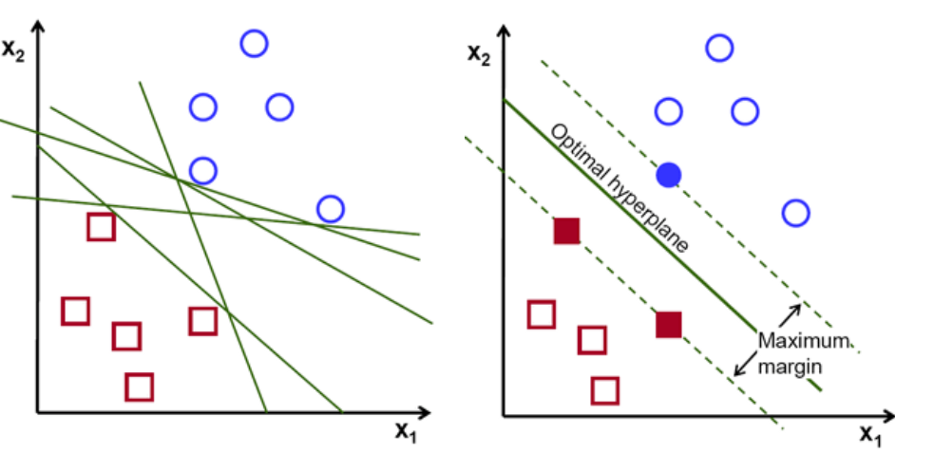
\includegraphics[scale=0.4]{Figs/optimal_hyperplane.png}
				\caption{Maximal Separating Hyperplane, \href{https://miro.medium.com/max/875/1*06GSco3ItM3gwW2scY6Tmg.png}{Source}}
			\end{figure}
		
			\item \tc{keywords}{Maximal (Optimal) Separating  Hyperplane}: 
			The separating hyperplane with the largest between-class margin \textbf{$M$}.
			\begin{equation*}
				\begin{aligned}
					\max_{\beta,\beta_0,M} \quad & M\\
					\textrm{s.t.} \quad & \sum_{j=1}^{p}{\beta_j^2 = 1}\\
					&distance: y^{(i)}(\beta^T x^{(i)} + \beta_0) \geq M \quad \forall i \in \{1,2,...,N\}   \\
				\end{aligned}
			\end{equation*}
			
		\end{itemize}	
		
	}
	
	\frame{\frametitle{Maximal Margin Classifier: Quadratic Program}
		
		
		\begin{itemize}
			\item Eq.(1) can be rephrased as a \tc{keywords}{convex quadratic problem} and be solved efficiently using QP solvers.
			\newline
			\item
			(Euclidean) distance between two hyperplanes \newline
			
			$$\mathcal{H}_1 = \{x | \beta^T x + \beta_0 = 1\} \quad \quad
			\mathcal{H}_2 = \{x | \beta^T x + \beta_0 = -1\}$$ \vspace{1mm}
			
			is \textbf {dist($\mathcal{H}_1, \mathcal{H}_2$)} = 2/$||\beta||_2$ \newline \newline
			
			\noindent\begin{minipage}{0.28\textwidth}
				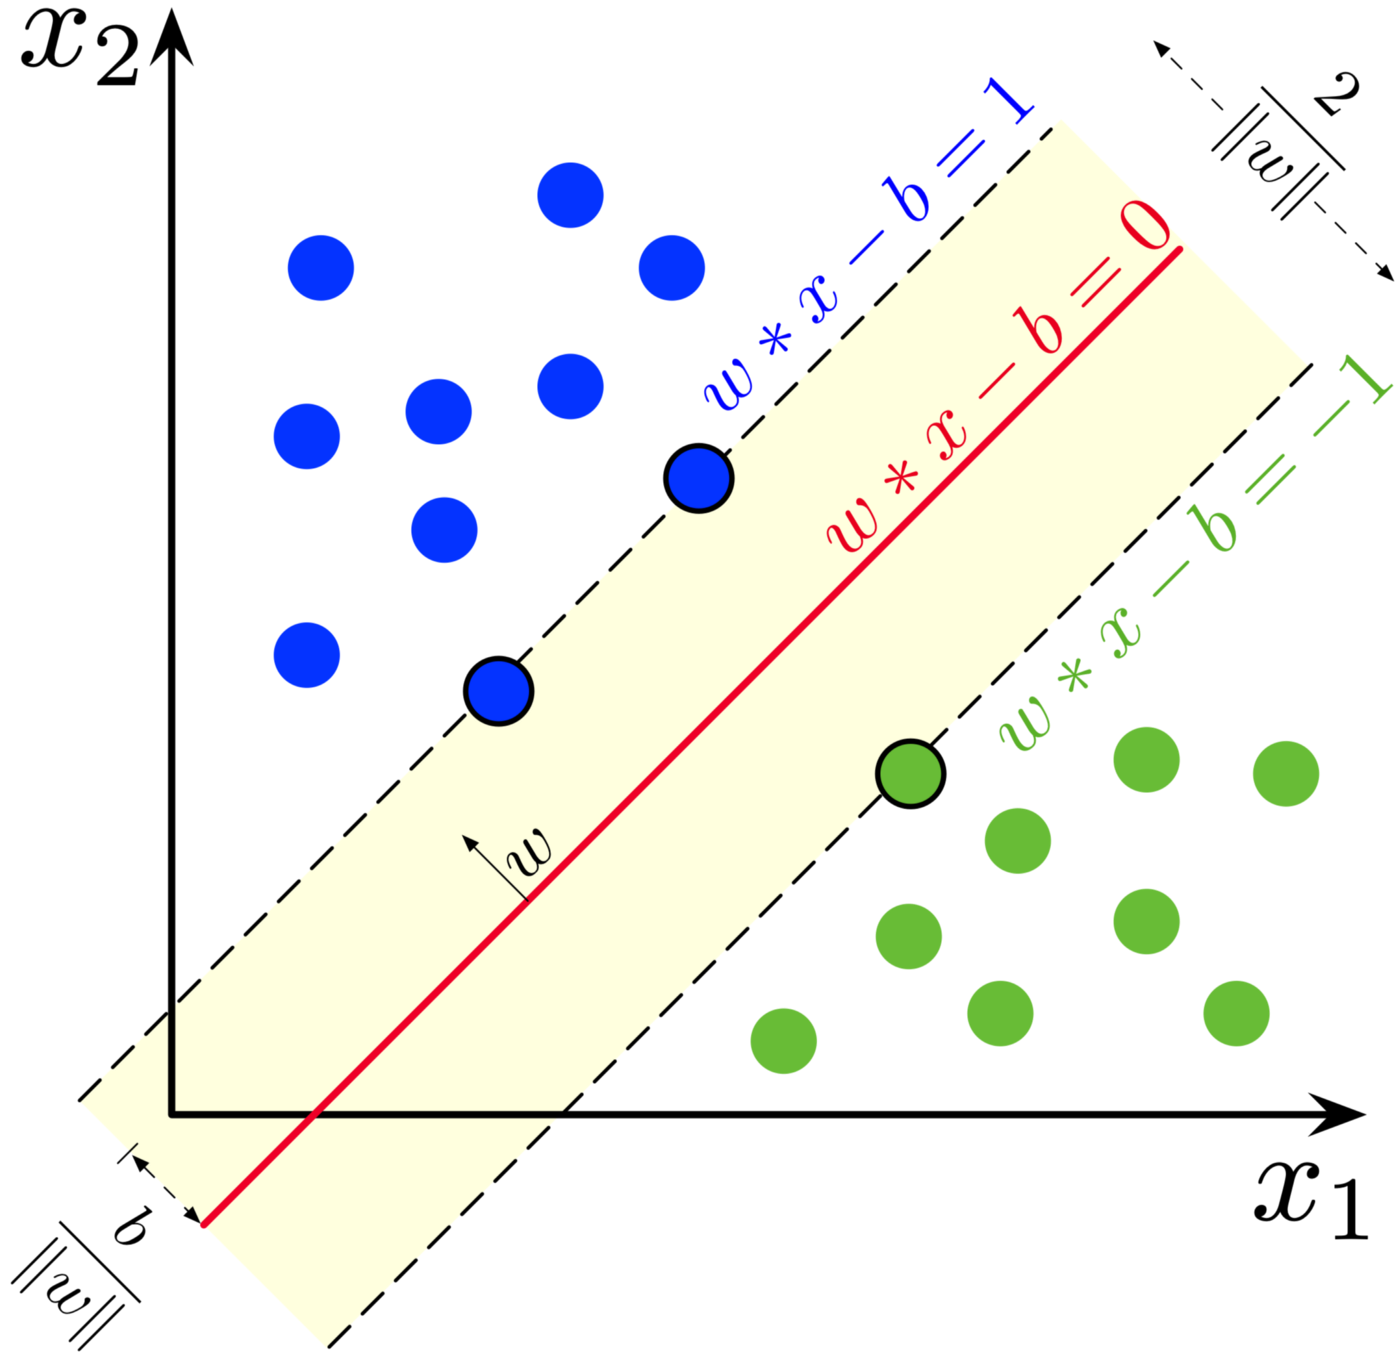
\includegraphics[width=\linewidth]{Figs/maximal_hyperplane.png}
				\captionof{figure}{Optimal Hyperplane, \href{https://commons.wikimedia.org/wiki/File:SVM_margin.png}{Source}}
			\end{minipage}
			\hfill
			\begin{minipage}{0.65\textwidth}\raggedleft
				\begin{equation*}
						\begin{aligned}
							\min_{\beta,\beta_0} \quad & \frac{1}{2}||\beta||_2 ^2\\
							\textrm{s.t.} \quad & y^{(i)}(\beta^T x^{(i)} +\beta_0) \geq 1 \quad \forall i \in \{1,2,...,N\}\\
						\end{aligned}
					\end{equation*}
			\end{minipage}
			
		\end{itemize}	
		
	}

	%%%%%%%%%%%%%%%%%%%%%%%%%%%%%%%%%%%%%%%%%%%%%%%%%%%%%%%%%%%%%%%%%%%
	\section{Support Vector Classifier}
	%%%%%%%%%%%%%%%%%%%%%%%%%%%%%%%%%%%%%%%%%%%%%%%%%%%%%%%%%%%%%%%%%%%
	\frame{\frametitle{Not-linearly Separable Data}
		
		\begin{itemize}
			
			\item In most cases however, the data are not linearly separable.
			\newline
			\begin{figure}
				\centering
				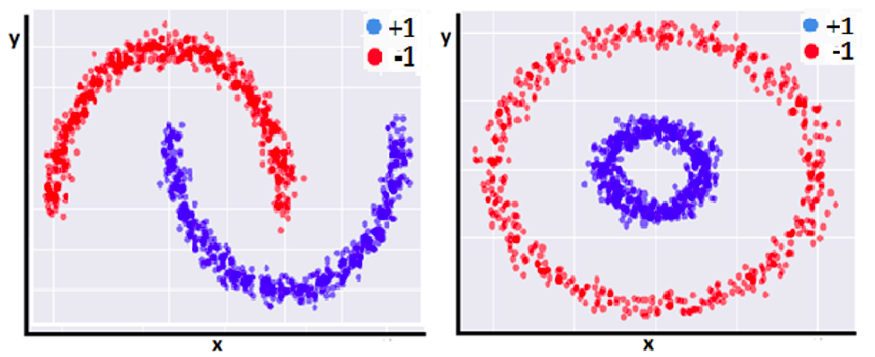
\includegraphics[scale=0.35]{Figs/nonlinear_datasets.png}
				\caption{Not-linearly Separable Data, \href{https://miro.medium.com/max/875/1*1o_4zV7Js_65TThqlDeGsg.png}{Source}}
			\end{figure}
			
		\end{itemize}	
		
	}

	\frame{\frametitle{Noisy Data}
		
		\begin{itemize}
			
			\item Sometimes the data are linearly separable, but noisy. This can lead to a poor solution for the maximal margin classifier. Also, hard-margin classifier is sensitive to \tc{keywords}{outliers}.
			\begin{figure}
				\centering
				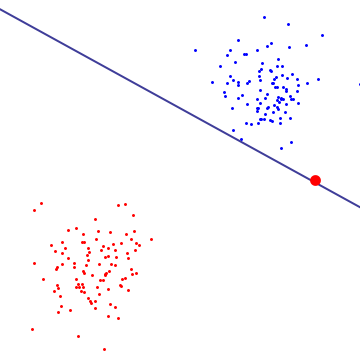
\includegraphics[scale=0.4]{Figs/outlier_effect_svm.png}
				\caption{Noisy Data, \href{https://qph.cf2.quoracdn.net/main-qimg-fd1abee68f789a96e0b706bd5bba3bb5}{Source}}
			
			\end{figure}
		
			\item \textcolor{Blue}{\textit {Support Vector Classifier} (SVC)} maximizes a \tc{keywords}{soft} margin.
			
		\end{itemize}	
		
	}


	\frame{\frametitle{Support Vector Classifier (Soft Margin Classifier)}
		
		\begin{itemize}
			
			\item Allowing some samples to violate the margin, with \tc{keywords}{slack variables ($\xi$)}, in a controlled manner:
			\begin{figure}
				\centering
				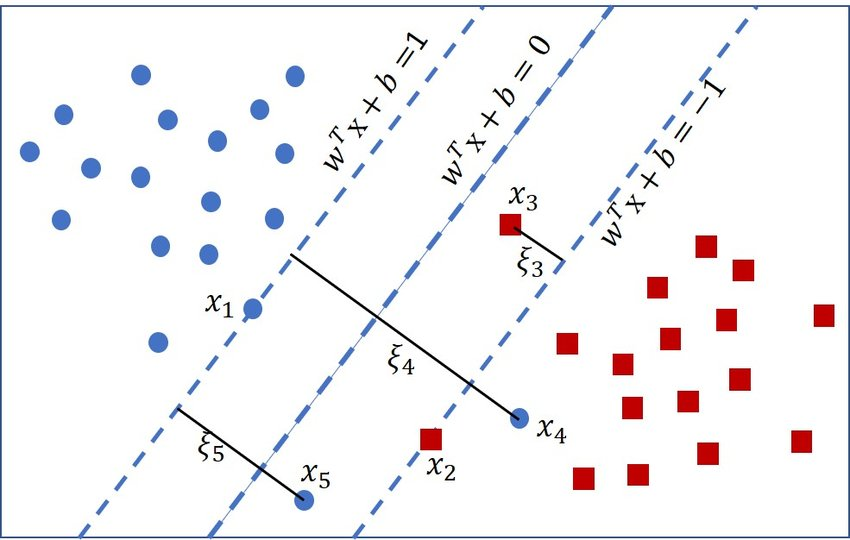
\includegraphics[scale=0.4]{Figs/soft_svm.png}
				\caption{Soft Margin Classifier, \href{https://www.researchgate.net/profile/Toan-Tran-28/publication/327015448/figure/fig2/AS:659696117633025@1534295219130/SVM-with-soft-margin-kernel-with-different-cases-of-slack-variables.png}{Source}}
			\end{figure}
			
			\begin{equation*}
				\begin{aligned}
					\min_{\beta,\beta_0,\xi} \quad & \frac{1}{2}||\beta||_2 ^2+C\sum_{i=1}^{N}{\xi_{i}}\\
					\textrm{s.t.} \quad & y^{(i)}(\beta^T x^{(i)} + \beta_0) \geq 1-\xi_{i}\\
					&\xi_i\geq0 \quad \forall i \in \{1,2,...,N\}   \\
				\end{aligned}
			\end{equation*}
			
		\end{itemize}	
		
	}


	\frame{\frametitle{Effect of Regularization Parameter}
		
		\begin{itemize}
			
			\item \textit C is a regularization parameter that controls the \tc{keywords}{width of the margin} in the support vector classifier.
			\begin{figure}
				\centering
				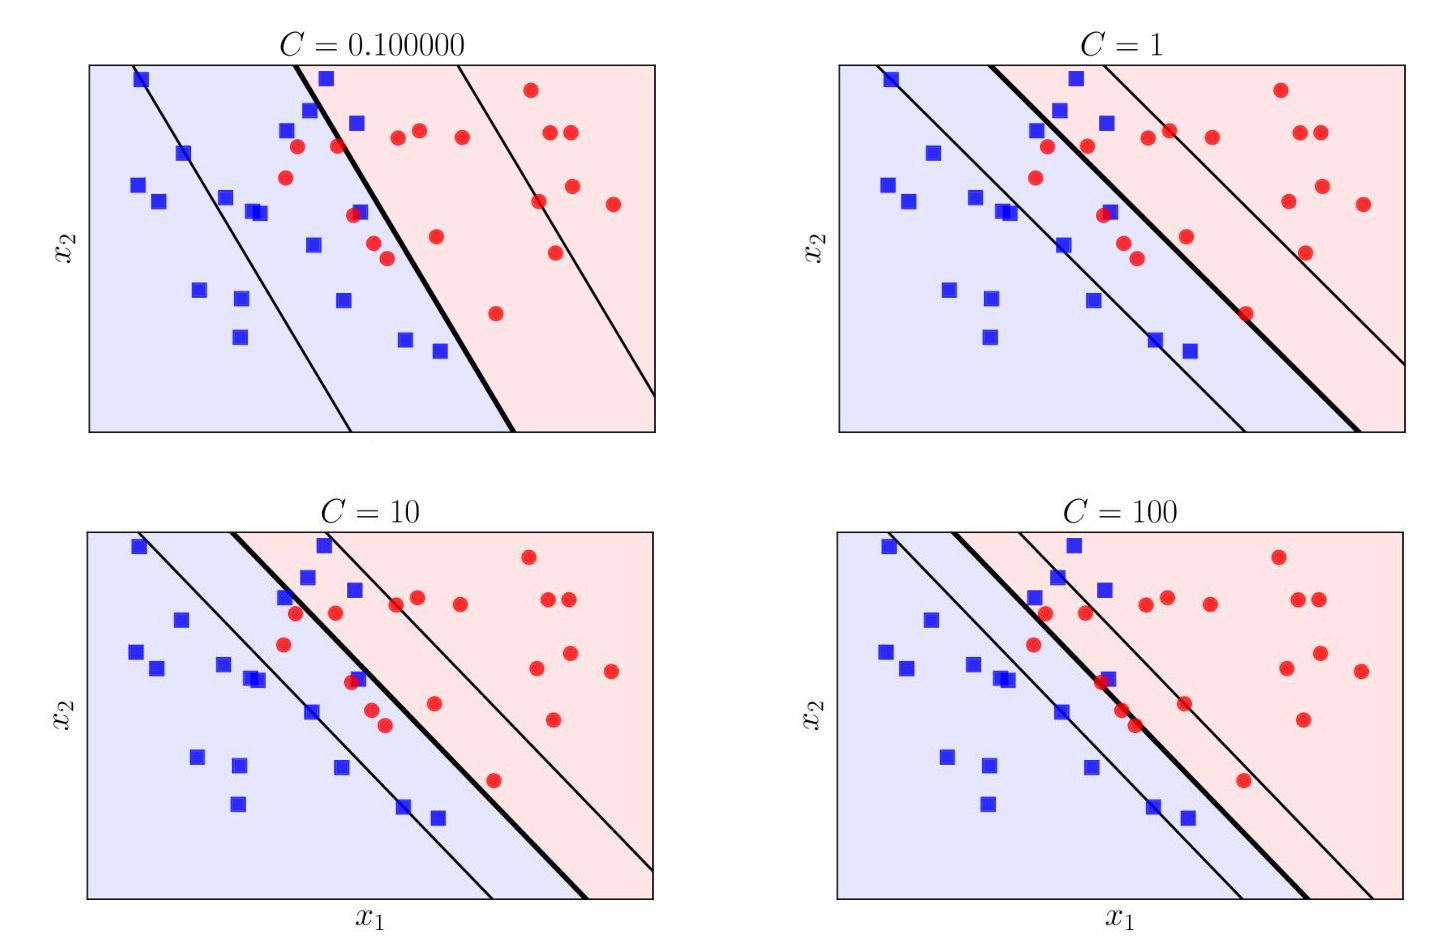
\includegraphics[scale=0.3]{Figs/regularization_parameter1.png}
				\caption{Regularization Effect, \href{https://dinhanhthi.com/img/post/ML/support-vector-machine/svm-7.jpg}{Source}}
			\end{figure}
			
		\end{itemize}	
		
	}


	\frame{\frametitle{Dual Problem of SVC}
		
		\begin{itemize}
			
			\item \textbf {Primal problem}:
			\begin{equation*}
				\begin{aligned}
					\min_{\beta,\beta_0,\xi} \quad & \frac{1}{2}||\beta||_2 ^2+C\sum_{i=1}^{N}{\xi_{i}}\\
					\textrm{s.t.} \quad & y^{(i)}(\beta^T x^{(i)} + \beta_0) \geq 1-\xi_{i}\\
					&\xi_i\geq0 \quad \forall i \in \{1,2,...,N\}   \\
				\end{aligned}
			\end{equation*}
			\newline
			
			\item \textbf {Dual problem} (using the lagrangian):
			\begin{equation*}
				\begin{aligned}
					\max_{\alpha_i} \quad & \sum_{i=1}^{N}{\alpha_i} - \frac{1}{2} \sum_{i=1}^{N}{\sum_{j=1}^{N} {\alpha_i \alpha_j y^{(i)} y^{(j)} \textcolor{Blue}{x^{{(i)}^T} x^{(j)}}}} \\
					\textrm{s.t.} \quad & \sum_{i=1}^{N} \alpha_i y^{(i)} = 0\\
					&0 \leq \alpha_i \leq C \quad \forall i \in \{1,2,...,N\}
					\\
				\end{aligned}
			\end{equation*}
		
			%\item We only need inner products!
			
		\end{itemize}	
		
	}


	\frame{\frametitle{KKT Conditions}
		
		\begin{itemize}
			
			\item From Karush-Kuhn-Tucker (KKT) conditions and complementary slackness we have:
			\begin{equation*}
				\begin{aligned}
					\alpha_i (1-\xi_i-y^{(i)}(\beta^Tx^{(i)} + \beta_0)) = 0\\
					(C - \alpha_i)\xi_i = 0\\
				\end{aligned}
			\end{equation*}
			\newline
			
			\item There can be 3 cases:
			\newline\\
			\begin{cases}
			$$\textcolor{Blue}{\alpha_i = 0} \rightarrow \textcolor{Red}{\xi_i = 0} \Rightarrow \textcolor{newcolor2}{1-y^{(i)}(\beta^T x^{(i)} + \beta_0) < 0} $$ : \qquad \text{Non-Support} \\
			 
			\newline\\
			$$\textcolor{Blue}{0 < \alpha_i < C} \rightarrow \textcolor{Red}{\xi_i = 0} \Rightarrow \textcolor{newcolor2}{1-y^{(i)}(\beta^T x^{(i)} + \beta_0) = 0} $$ : \quad \text{Support} \\
			
		    \newline\\
			$$\textcolor{Blue}{\alpha_i = C} \rightarrow \textcolor{Red}{\xi_i > 0} \Rightarrow \textcolor{newcolor2}{1- \xi_i - y^{(i)}(\beta^T x^{(i)} + \beta_0) = 0} $$ : \quad \text{Support} \\ 
			\end{cases}
			
		\end{itemize}	
		
	}

	\frame{\frametitle{Classification Function}
		
		\begin{itemize}
			
			\item $f(x) = \beta^T x + \beta_0$
			\newline
			\item Also, when minimizing the conjugate function of primal problem, we get: $$\beta = \sum_{i=1}^{N}{\alpha_i y^{(i)}x^{(i)}}$$
			
			\item This results in the following classification function for SVC:
			\begin{equation*}
					f(x) = \beta_0 + \sum_{i=1}^{N} \alpha_i y^{(i)} \textcolor{Blue}{x^T x^{(i)}} = \beta_0 + \sum_{i=1}^{N} \alpha_i y^{(i)} \textcolor{Blue}{\langle x, x^{(i)} \rangle}
			\end{equation*}
			
			\item It turns out that most of the $\hat{\alpha}_i$ can be zero:
			\begin{equation*}
				f(x) = \beta_0 + \sum_{i \in \mathcal{S}} \hat{\alpha}_i y^{(i)} \textcolor{Blue}{\langle x, x^{(i)} \rangle}
			\end{equation*}
			where \tc{keywords}{$\mathcal{S}$} is the \tc{keywords}{support set} of indices $i$ such that $\hat{\alpha}_i > 0$. \newline \newline
			So, all we need is \tc{keywords}{inner products}!
			
		\end{itemize}	
		
	}


	\section{Support Vector Machines}
	%%%%%%%%%%%%%%%%%%%%%%%%%%%%%%%%%%%%%%%%%%%%%%%%%%%%%%%%%%%%%%%%%
	
	\frame{\frametitle{The Need for Non-Linear Boundary}
		
		\begin{itemize}
			
			\item Linear boundary can fail in many cases, regardless of the value of C.
			\newline
			\begin{figure}
				\centering
				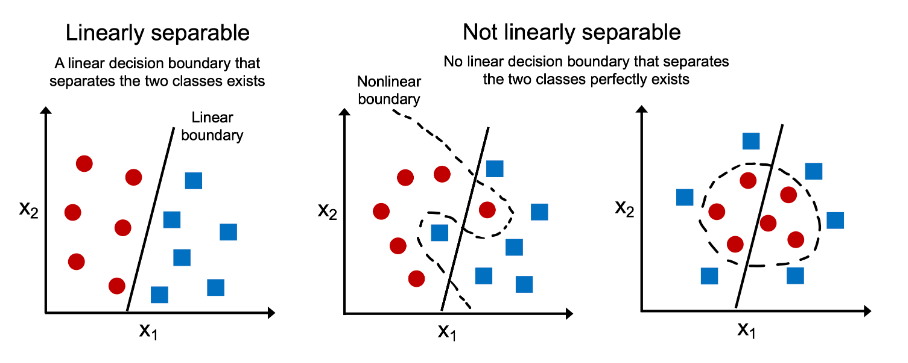
\includegraphics[scale=0.7]{Figs/Linearly-vs-Not-linearly-separable-datasets.png}
				\caption{The Need for Non-linear Boundary , \href{https://vitalflux.com/wp-content/uploads/2022/04/Linearly-vs-Not-linearly-separable-datasets.png}{Source}}
			\end{figure}
			
		\end{itemize}	
		
	}

	\frame{\frametitle{Feature Expansion}
		
		\begin{itemize}
			
			\item Enlarge the space of features by including transformations;
			e.g. $X_1^2 , X_1^3, X_1X_2, X_1X_2^2,...$ . Hence increasing the dimension of the original \textit p-dimensional input space.
			\newline
			\item Then we can fit a support vector classifier in the enlarged space.
			\newline
			\item This results in \tc{keywords}{non-linear decision boundaries} in the original feature space.
			
			\begin{figure}
				\centering
				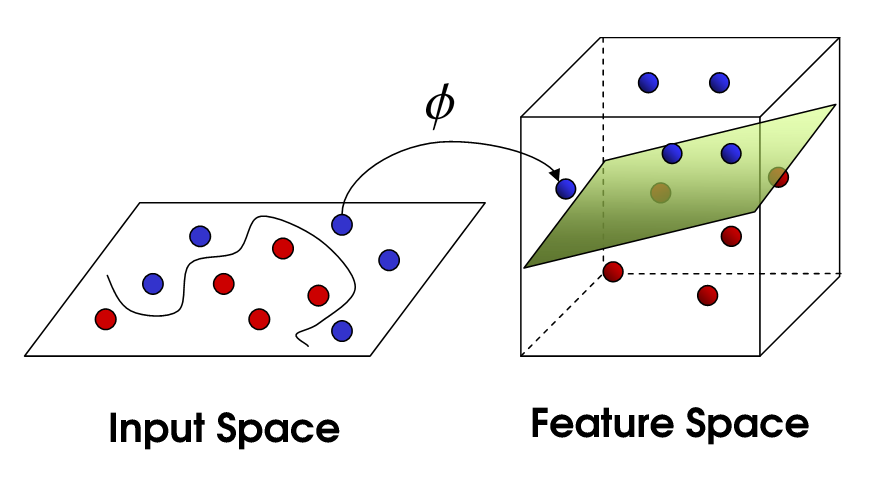
\includegraphics[scale=0.25]{Figs/feature_expansion.png}
				\caption{The Need for Non-inear Boundary , \href{https://miro.medium.com/max/875/1*zWzeMGyCc7KvGD9X8lwlnQ.png}{Source}}
			\end{figure}
			
		\end{itemize}	
		
	}


	\frame{\frametitle{Kernels and SVMs}
		
		\begin{itemize}
			
			\item Consider the feature mapping $T: x \rightarrow \phi(x)$, we define the corresponding \tc{keywords}{kernel} to be 
			\begin{equation*}
				K(x, x') = \langle \phi(x),\phi(x') \rangle .
			\end{equation*}
			
			Now we can simply replace all inner products by $ K(x, x')$, and our algorithm would now be learning using the features $\phi$. \newline \newline
			
			\item Kernel matrix: $\quad K_{i,j} = K(x^{(i)}, x^{(j)})$
			
			A valid kernel function is the one that results in a \tc{keywords}{symmetric positive semi-definite} kernel matrix for any set of samples. (\textit{Mercer theorem}: necessary and sufficient condition) \newline \newline
			
			\item Calculating kernel matrix may be very \tc{keywords}{inexpensive}, even though $\phi(x)$ itself may be very expensive to calculate (perhaps because it is an extremely high dimensional vector).\newline \newline
			
			\item The classification function solution has the form
			\begin{equation*}
				f(x) = \beta_0 + \sum_{i \in \mathcal{S}} \hat{\alpha}_i y^{(i)} \textcolor{Blue}{K(x,x^{(i)})}
			\end{equation*}
			
		\end{itemize}	
		
	}

	\frame{\frametitle{Polynomial Kernels}
		
		\begin{equation*}
			K(x,y) = (1+\langle x,y \rangle)^d
		\end{equation*}
	
		\begin{itemize}
			
			\item e.g. Feature transformation from 2D kernels:
				$$K(x,y) = (1+\langle x,y \rangle)^2 \Rightarrow \phi(x) = (1, \sqrt{2}x_1, \sqrt{2}x_2, x_1^2, x_2^2)$$
		
			\begin{figure}
					\centering
					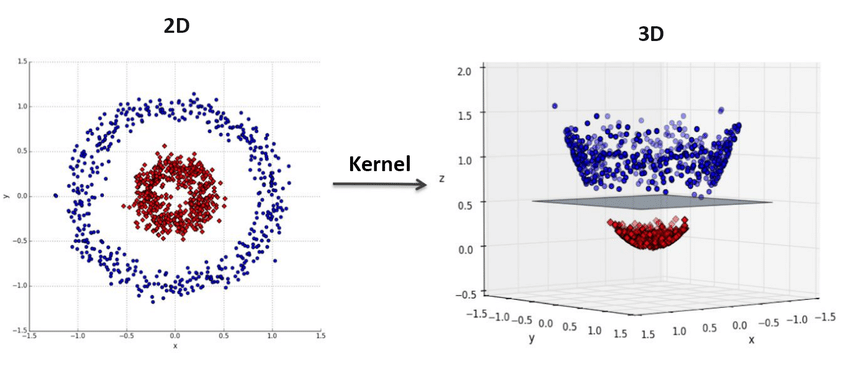
\includegraphics[scale=0.35]{Figs/poly2_kernel_svm.png}
					\caption{2nd Order Polynomial Kernel, \href{https://www.researchgate.net/profile/Marouane-Hachimi/publication/340610860/figure/fig4/AS:880021191286786@1586824810950/Non-linear-classifier-using-Kernel-trick-16.ppm}{Source}}
			\end{figure}
			
			
		\end{itemize}	
		
	}
	
	\frame{\frametitle{Radial Basis Kernels}
		
		\begin{equation*}
			K(x,y) = \exp(-\gamma \lVert x-y \rVert_2 ^2)
		\end{equation*}
		
		\begin{itemize}
		
			\item Measure of similarity!
			\item $\gamma$ is the hyperparameter to be chosen to control the bias-variance trade-off.
			
			\begin{figure}
				\centering
				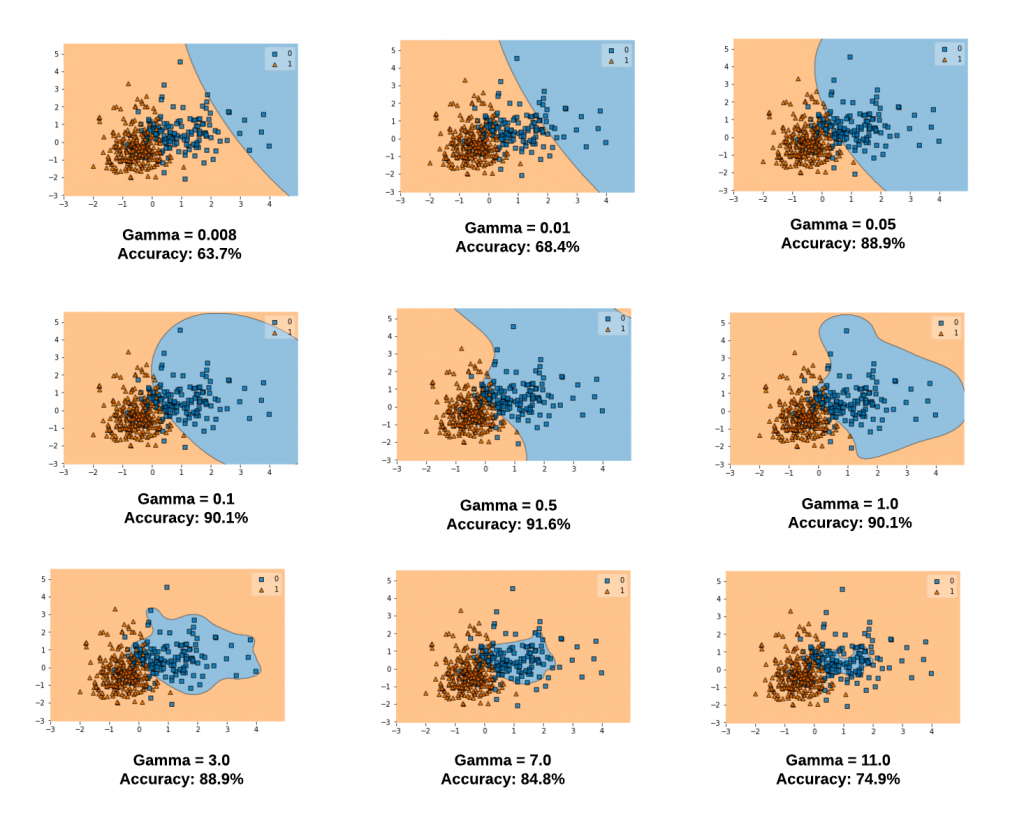
\includegraphics[scale=0.25]{Figs/rbf_kernel_svm1.png}
				\caption{RBF Kernel, \href{https://vitalflux.com/wp-content/uploads/2020/07/C-Values-Page-3-1024x832.png}{Source}}
			\end{figure}
			
		\end{itemize}	
		
	}

	\frame{\frametitle{Multi-class SVM}
		
		\begin{itemize}
			
			\item \tc{keywords}{One-vs-All}: Fit all $K$ different 2-class SVM classifiers $\hat{f}_{k}(x), \forall k\in \{1,2,...,K\}$; each class versus the rest. Classify $x^*$ to the class for which $\hat{f}_{k}(x)$ is the largest. \newline
			
			\item \tc{keywords}{One-vs-One}: Fit all ${K \choose 2}$ pairwise classifiers $\hat{f}_{kl}(x)$. Classify $x^*$ to the class that wins the most pairwise competitions. \newline
			
			\begin{figure}
					\centering
					\subfloat[\centering One-vs-All]{{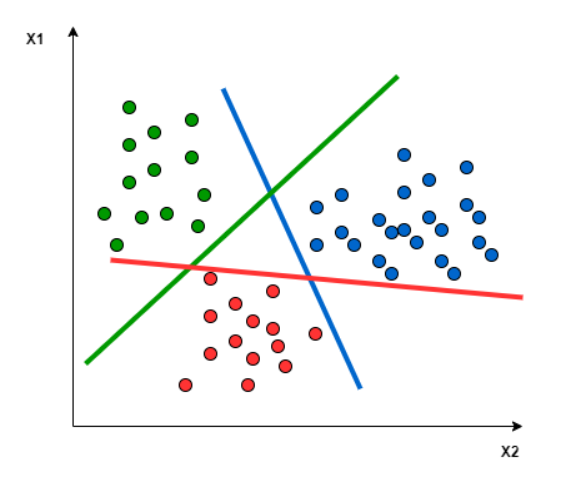
\includegraphics[scale=0.4]{Figs/ova.png} }}%
					\qquad
					\subfloat[\centering One-vs-One]{{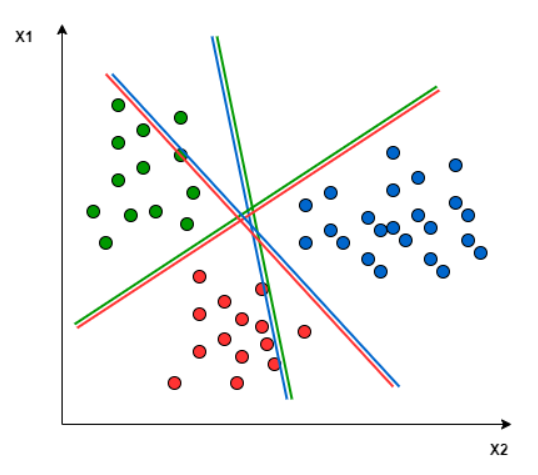
\includegraphics[scale=0.4]{Figs/ovo.png} }}
					\caption{Multi-class SVM, \href{https://www.baeldung.com/cs/svm-multiclass-classification}{Source}}
			\end{figure}
			
			
		\end{itemize}	
		
	}

	\frame{\frametitle{Support Vector Regression}
		
		\begin{itemize}
			
			\begin{figure}
					\centering
					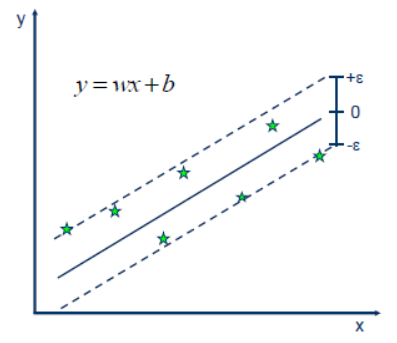
\includegraphics[scale=0.6]{Figs/svr.png}
					\caption{Support Vector Regression, \href{https://www.saedsayad.com/support_vector_machine_reg.htm}{Source}}
			\end{figure}
		
			\begin{equation*}
				\begin{aligned}
					\min_{\beta,\beta_0} \quad & \frac{1}{2} ||\beta||_2 ^2\\
					\textrm{s.t.} \quad & |y^{(i)} - (\beta^T x^{(i)} + \beta_0)|_2 \leq \epsilon \quad \forall i \in \{1,2,...,N\}\\
				\end{aligned}
			\end{equation*}
			
			
		\end{itemize}	
		
	}


	\frame{\frametitle{Soft Support Vector Regression}
		
		\begin{itemize}
			
			\begin{figure}
					\centering
					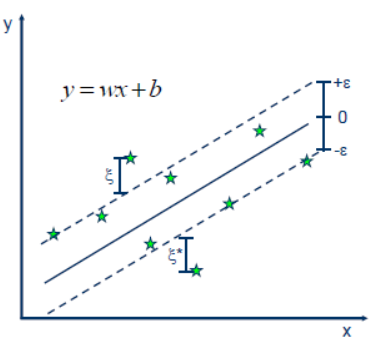
\includegraphics[scale=0.6]{Figs/soft_svr.png}
					\caption{Soft Support Vector Regression, \href{https://www.saedsayad.com/support_vector_machine_reg.htm}{Source}}
			\end{figure}
			
			\begin{equation*}
				\begin{aligned}
					\min_{\beta,\beta_0} \quad & \frac{1}{2} ||\beta||_2 ^2 + C\sum_{i=1}^{N}{\xi_i}\\
					\textrm{s.t.} \quad & |y^{(i)} - (\beta^T x^{(i)} + \beta_0)|_2 \leq \epsilon + \xi_i \\
					&\xi_i \geq 0 \quad \forall i \in \{1,2,...,N\}\\
				\end{aligned}
			\end{equation*}
			
			
		\end{itemize}	
		
	}

	
	
	%%%%%%%%%%%%%%%%%%%%%%%%%%%%%%%%%%%%%%%%%%%%%%%%%%%%%%%%%%%%%%%%%%%
	\frame{\frametitle{Final Notes}
			\centering
			\vspace{50 pt}
			\textbf{Thank You!}
			\vspace{50pt}
			
			\textbf{Any Question?}
		}
	%%%%%%%%%%%%%%%%%%%%%%%%%%%%%%%%%%%%%%%%%%
\end{document}